\documentclass{entcs} 
\usepackage{entcsmacro}
\usepackage{graphicx}
\usepackage{code,amsmath,amssymb,math-cmds}

\newcommand{\cut}[1]{}

\newcommand{\appref}[1]{Appendix~\ref{#1}}
\newcommand{\secref}[1]{Section~\ref{#1}}
\newcommand{\tblref}[1]{Table~\ref{#1}}
\newcommand{\figref}[1]{Figure~\ref{#1}}
\newcommand{\listingref}[1]{Listing~\ref{#1}}
%\newcommand{\pref}[1]{{page~\pageref{#1}}}

\newcommand{\eg}{{\em e.g.}}
\newcommand{\cf}{{\em cf.}}
\newcommand{\ie}{{\em i.e.}}
\newcommand{\etc}{{\em etc.\/}}
\newcommand{\naive}{na\"{\i}ve}
\newcommand{\role}{r\^{o}le}
\newcommand{\forte}{{fort\'{e}\/}}
\newcommand{\appr}{\~{}}

\newcommand{\bftt}[1]{{\ttfamily\bfseries{}#1}}
\newcommand{\kw}[1]{\bftt {#1}}
\newcommand{\Pthen}{\kw{Pthen}}
\newcommand{\pads}{\textsc{pads}}
\newcommand{\padsl}{\textsc{padsl}}
\newcommand{\padst}{\textsc{pads/t}}
\newcommand{\datatype}{\textsc{PADS/T}}
%\newcommand{\datatype}{\textsc{DataType}}
\newcommand{\C}{\textsc{C}}
\newcommand{\perl}{\textsc{Perl}}
\newcommand{\ml}{\textsc{ml}}
\newcommand{\sml}{\textsc{sml}}
\newcommand{\smlnj}{\textsc{sml/nj}}
\newcommand{\java}{\textsc{java}}
\newcommand{\ddl}{\textsc{ddl}}
\newcommand{\xml}{\textsc{xml}}
\newcommand{\datascript}{\textsc{DataScript}}
\newcommand{\packettypes}{\textsc{PacketTypes}}
\newcommand{\erlang}{\textsc{Erlang}}

\newcommand{\Core}{Ad hoc}
\newcommand{\core}{ad hoc}
\newcommand{\pvalue}{\core{} value}
\newcommand{\ppat}{\core{} pattern}
\newcommand{\ptype}{\core{} type}

\newcommand{\padsc}{\textsc{pads}/\C{}}
\newcommand{\padsml}{\textsc{pads}/\ml{}}

\newcommand{\dibbler}{Sirius}
\newcommand{\ningaui}{Altair}
\newcommand{\darkstar}{Regulus}

\newcommand{\pdgood}{{\tt G}}
\newcommand{\pdbad}{{\tt B}}
\newcommand{\pdnest}{{\tt N}}
\newcommand{\pdsem}{{\tt S}}
\newcommand{\ptypes}{T}
\newcommand{\patreadpd}[2]{{\tt #1<<#2>>}}
\newcommand{\btm}{\cd{BOT}}


\newcommand{\lsem}{{[\![}}
\newcommand{\rsem}{{]\!]}}


\newcommand{\figHeight}[4]{\begin{figure}[tb]
	\centerline{
	            \epsfig{file=#1,height=#4}}
	\caption{#2}
	\label{#3}
	\end{figure}}

%% Environment for typesetting BNF grammars. Uses display math mode.
\newenvironment{bnf}
     {%% local command definitions:
        %% BNF definition symbol
      \def\->{\rightarrow}
%%      \def\::={{::=} &}
      \def\::={\bnfdef &}
      \def\|{\bnfalt}
      \newcommand{\name}[1]{\text{##1}}
        %% non-terminal
      \newcommand{\nont}[1]{{##1}}
      \newcommand{\meta}[1]{& ##1 &}
      \newcommand{\descr}[1]{& \text{// ##1}}
      \newcommand{\opt}[1]{ [##1] }
      \newcommand{\opnon}[1]{\opt{\nont{##1}}}
      \newcommand{\none}{\epsilon}
      \newcommand{\nwln}{\\ &&&}
      \newcommand{\nlalt}{\\ && \| &}
      \[\begin{array}{lrlll}
     }
     {\end{array}\]}

\newcommand{\mcd}[1]{\mathtt{#1}}
\newcommand{\ppair}[3]{#1{:}#2 \mathrel{**} #3}
\newcommand{\parray}[3]{#1\;\mcd{Parray}(#2,#3)}
\newcommand{\pset}[3]{\{#1{:}#2\,|\,#3\}}
\newcommand{\pstream}[1]{#1\;\mcd{stream}}
\newcommand{\precord}[1]{\{\{#1\}\}}


% A couple of exemplary definitions:
\def\lastname{Fernandez, Fisher, Mandelbaum and Walker}
\begin{document}
\begin{frontmatter}
  \title{\datatype{}: Language Support for Processing Ad Hoc Data Sources} 
  \author{Maria Fernandez,
    Kathleen Fisher\thanksref{attemail}}
  \address{AT\&T\\ 
    Florham Park,NJ USA} 
  \author{Yitzhak Mandelbaum,
    David Walker\thanksref{premail}}
  \address{Department of Computer Science\\ 
    Princeton University\\
    Princeton,NJ USA} 
  \thanks[attemail]{Email:\texttt{\normalshape
        mff,kfisher@research.att.com}}
  \thanks[premail]{Email:\texttt{\normalshape
        yitzhakm,dpw {\it at} cs {\it dot} princeton {\it dot} edu}}
\begin{abstract} 
  Insert abstract here.
\end{abstract}
\begin{keyword}
  Please list keywords from your paper here, separated by commas.
\end{keyword}
\end{frontmatter}

\section{Introduction}
\label{intro}

An {\em ad hoc data format} is any nonstandard data format for which
parsing, querying, analysis or transformation tools are not readily
available.  \xml{} is not an ad hoc data format --- there are hundreds
of tools for reading, querying, and transforming \xml{}.  However,
computer programmers, financial analysts, computational biologists,
chemists and physicists, healthcare and airline information systems,
corporate IT professionals and others deal with deal ad hoc data in a
myriad of complex formats on a daily basis.  This data is often
unpredictable, poorly documented, and filled with errors, making it
extremely difficult to deal with.  Often, before anything can be done
with ad hoc data one must clense it of as many errors as possible,
normalize its shape and transform it into a standardized format.  Once
in a standardized format, the data can be directly loaded into a
database or manipulated by standard, widely available tools.

% The goal of this paper is to describe a new language for efficient and
% reliable computing with ad hoc data.  More specifically, we describe a
% high-level programming language, \datatype{}, that comes with
% intrinsic support for processing ad hoc data.  Our programming
% language will use the rich data descriptions both as directives for
% parsing ad hoc data sources and as types for describing
% representations of ad hoc data within the programming environment.  In
% addition, a critical facet of our language will be its support for
% {\em error-aware computing}.  Our error-aware infrastructure will
% allow programmers to conveniently verify correctness of data relative
% to a description or alternatively detect data errors and handle them
% in domain-specific ways.  Finally, we will be sure our language design
% is founded on strong programming language principles by studying its
% type system and metatheory extensively.

There are vast amounts of useful data stored in traditional databases
and \xml{} formats, but there is just as much in ad hoc formats.
\figref{figure:data-sources} provides some information on ad hoc data
formats from the networking and telecommunications domain at AT\&T and
ad hoc data formats used by computational biologists at Princeton.
They include ASCII, binary, and Cobol data formats, with both fixed
and variable-width records arraged in linear sequences or in tree- or
DAG-shaped hierarchies.  The data sources range in size from
relatively small files up to network applications, such as web server
logs, which can be produced at a rate of 12GB per week, to Netflow
applications, which can be produced at over one GB per second.  Common
errors include undocumented data, corrupted data, missing data, and
multiple missing-value representations.

We hope that these examples give the reader a beginning sense of the
nature and pervasiveness of ad hoc data sources.  However, we cannot
emphasize enough just how pervasive ad hoc data is and to what degree
it infiltrates computer systems, businesses, government, and
scientific research.  Remember, just about any program that spits out
useful information in a format other than \xml{}, \textsc{html},
\textsc{jpeg}, \textsc{mpeg} or a few others is generating ad hoc
data.  Hence, most programmers deal with ad hoc data on a individual
basis regularly.  When it comes to ad hoc data on a grand scale,
perhaps the most daunting challenge will come from the national
health-care system.  Recently, Newt Gingrich and Hilary Clinton have
jointly proposed we consolidate and integrate our national healthcare
records in the next 10 years.  Such a massive project will undoubtedly
require technical solutions at many levels.  At the lowest levels, we
will need a reliable software to collect and transfer health care data
from legacy systems into modern formats.  The \datatype{} system we
propose will be an invaluable aid in the development of this software.

\begin{figure*}
\begin{center}
\begin{tabular}{@{}|l|l|l|l|}
\hline
Name: Use                           & Representation    
%& Size
           & Common Errors \\ \hline\hline
Web server logs (CLF):                & Fixed-column      
%& $\leq$12GB/week 
& Race conditions on log entry\\ 
Measuring web workloads               & ASCII records     
%&                             
& Unexpected values\\ \hline
AT\&T provisioning data (\dibbler{}): & Variable-width    
%& 2.2GB/week 
& Unexpected values \\ 
Monitoring service activation         & ASCII records     
%&            
& Corrupted data feeds \\ \hline
Call detail:                   & Fixed-width       
%&\appr{}7GB/day 
&  Undocumented data\\
Fraud detection 
                                      & binary records  
%& 
& \\ \hline 
AT\&T billing data (\ningaui{}):      & Cobol  
%& \appr{}4000 files/day, 
& Unexpected values\\ 
Monitoring billing process   &                             
%& 250-300GB/day    
& Corrupted data feeds \\ \hline
IP backbone data (\darkstar{})  & ASCII  
%& $\ge$ 15 sources  
& Multiple missing-value rep's \\
Network Monitoring:  &        
%& \appr{}15 GB/day              
& Undocumented data \\ \hline
Netflow                               & Data-dependent      
%& $\ge$1Gigabit/second  
& Missed packets\\ 
Network Monitoring:        & number of   
%&                       
& \\
                                      & fixed-width 
%&
& \\
                                      & binary records 
%&
& \\ \hline
Gene Ontology data:        & Variable-width ASCII records 
%& ? 
&  \\
Gene-gene correlations in Magic & in DAG-shaped hiearchy 
%&  
& \\
database &
%& 
& \\\hline
Newick data                          & Fixed-width ASCII record 
%& ? 
& Manual entry errors \\
Immune system response simulation & in tree-shaped hierarchy 
%& 
& \\
\hline
\end{tabular}
\caption{Selected ad hoc data sources.}
\label{figure:data-sources}
\end{center}
\end{figure*}

Processing all this ad hoc data is challenging for a variety of
reasons.  First, ad hoc data typically arrives ``as is'': the analyst
or system that receives it can only say ``thank you,'' not request a
more convenient format.  Second, documentation for the format may not
exist at all, or it may be out of date.  A common phenomenon is for a
field in a data source to fall into disuse.  After a while, a new
piece of information becomes interesting, but compatibility issues
prevent data suppliers from modifying the shape of their data, so
instead they hijack the unused field, often failing to update the
documentation in the process.

Third, such data frequently contain errors for a variety of reasons:
malfunctioning equipment, race conditions on log entry~\cite{wpp},
non-standard values to indicate ``no data available,'' human error in
entering data, unexpected data values, \etc{} The appropriate response
to such errors depends on the application.  Some applications require
the data to be error free: if an error is detected, processing needs
to stop immediately and a human must be alerted.  Other applications
can repair the data, while still others either set data aside for a
human user to investigate or simply discard the erroneous or
unexpected values altogether.  For some applications, errors in the
data can be the most interesting part because they can signal where
two systems are failing to communicate.

A fourth challenge is that ad hoc data sources can be high volume:
AT\&T's call-detail stream contains roughly 300~million calls per day
requiring approximately 7GBs of storage space. Although this data is
eventually archived in a database, analysts mine it profitably before
such archiving~\cite{kdd98,kdd99}. More challenging, the \ningaui{}
project at AT\&T accumulates billing data at a rate of 250-300GB/day,
with occasional spurts of 750GBs/day. Netflow data arrives from Cisco
routers at rates over a gigabyte per second~\cite{gigascope}! Such
volumes mean it must be possible to process the data without loading
it all into memory at once.

A final challenge is that ad hoc data often needs to be translated
into a new, more useful or more standard format before anything can be
done with it.  Intuitively, this transformation can be done in three
stages.  First, one must generate a parser for the ad hoc format to
read it into a program.  Second, one must engineer the transformation
itself by filtering unwanted parts, normalizing representations, and
detecting and correcting or deleting erroneous data.  Third,
transformed data must be printed in the new format that can be
processed by standards tools.

Today, people tend to use \C{} or \perl{} for this task.
Unfortunately, writing parsers, transformations and printers this way
is tedious and error-prone, complicated by the lack of documentation,
convoluted encodings designed to save space, the need to produce
efficient code, and the need to handle errors robustly to avoid
corrupting down-stream data.  Moreover, the parser writers' hard-won
understanding of the data ends up embedded in parsing code, making
long-term maintenance difficult for the original writers and sharing
the knowledge with others nearly impossible.

Solution: Data description Language + transform language
Combine data description language with a transform language.
\pads{} is bound to C. However, functional programming languages are
better suited to the task of data tranformation. We therefore propose
a new language, \datatype{}, that combines a data description language
based on the style of ML types (and datatypes) with a functional data
transformation language. 

Our contributions are twofold. First, we propose an ML-style syntax
for the \pads{} data description language, based on type definitions
and {\em(polymorphic coming soon?)} parameterized recursive datatypes
(support for recursive datatypes is new to the \pads{} language, based
on recent results in our other work). This new syntax has a number of
advantages. It is more concise than the C-style encoding and more
naturally suited to describing recursive datatypes. Most importantly,
the new syntax is much more appropriate for transformation language
proposed below, which is based heavily on pattern-matching and data
constructors.

Our second contribution is the data transformation language itself.
{\em \pads{} is not a programming language.}  It merely generates
libraries that can be used by \C{} programmers.  \C{} is a very
low-level language that makes transforming ad hoc data awkward,
cumbersome and potentially error-prone.  More importantly, it provides
no intrinsic support for dealing with the errors that appear in ad hoc
data.  In addition, \C's type system and operational model provide no
support for checking the rich invariants found in ad hoc data either
at run time or at compile time.  In contrast, \datatype{} is a
high-level language with an elegant and convenient syntax for
data-driven programming, intrinsic support for handling errors and
intrinsic mechanisms for checking data invariants at run time {\em
  coming soon: and a sophisticated type system for enforcing data
  invariants at compile time}. 

At its core, \datatype{} is a functional language with standard
features such as pattern matching and higher-order functions, which we
view as critical to supporting data-driven transforms. In addition,
\datatype{} allows programmers to enforce semantic constraints on
data by using \datatype{} descriptions as a special form of runtime
contracts. The basic values of the language will be pairs of data
items and their corresponding meta-data. For each data item, the meta
data will include, among other things, descriptions of the error
content of the data item. Through the type system, the language will
ensure that data and associated meta data are kept in sync. This
property (which we call ``error-aware computing'') enables three
critical language features.
\begin{enumerate}
\item Safe, error-transparent transformations
\item Error querying - analyst can extract detailed picture of data
  error profile.
\item Flexible, programmatic repair of faulty records - analyst can
  choose when in the processing stream to address errors, rather than
  being forced to drop all faulty records at the beginning of the process.
\end{enumerate}

In the next section, we will describe, in detail, the \pads{} approach
to data and meta data (inherited by \datatype{}), the \datatype{}
syntax for data description, and illustrative examples. Next, in
section~\ref{sec:data-transformation} we will elaborate on
\datatype{}'s support for data transformation, including design,
syntax, brief overview of the semantics and some examples.
Section~\ref{sec:implementation-techniques} will discuss our proposed
implementation techiniques, and section~\ref{sec:related-work} the
related work. A discussion of conclusions and future work is included
in section~\ref{sec:conclusion}.


\subsection{Architecture}

\begin{figure}[tp]
  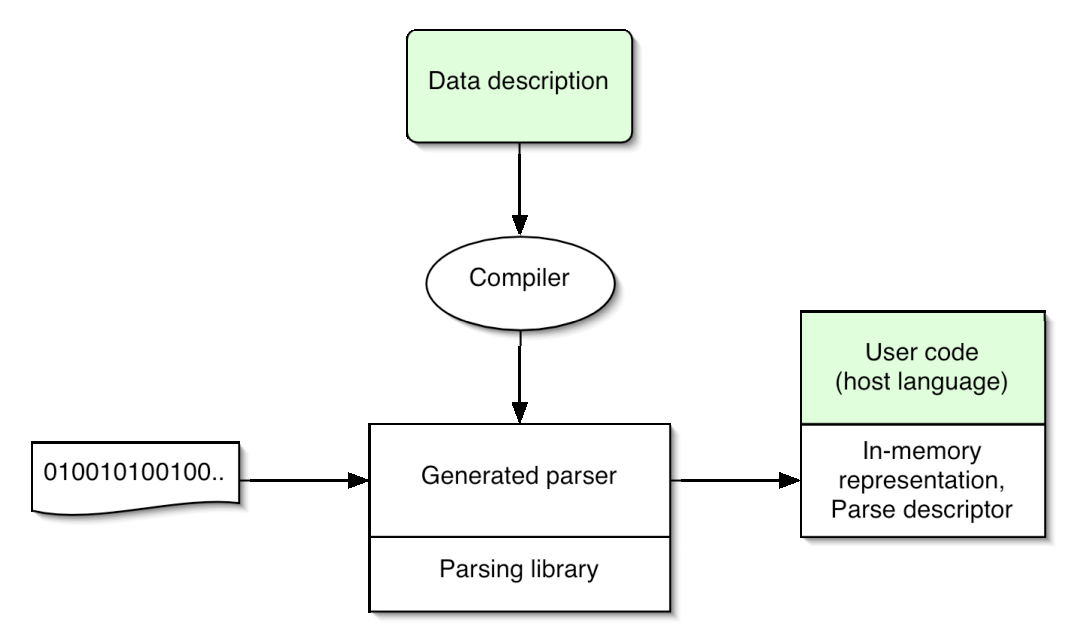
\includegraphics[height=3in,width=5in]{architecture.eps}
%  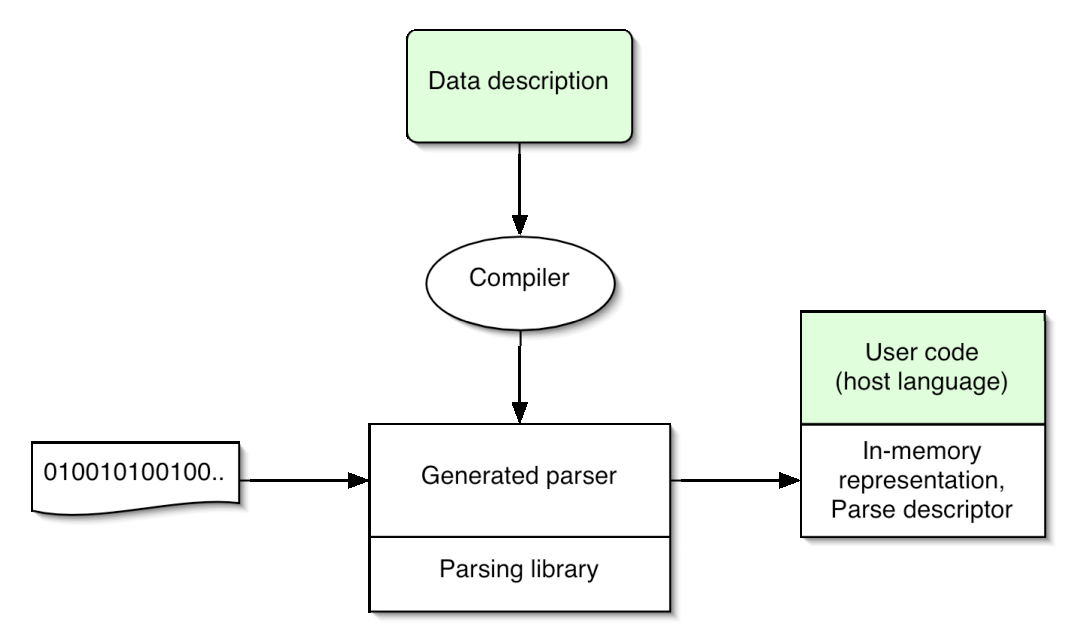
\includegraphics{architecture.eps}
\label{fig:pads-arch}
\caption{The \pads{} Architecture}
\end{figure}

\section{Describing Data in \datatype{}}
\label{sec:data-description}

%\datatype{} inherits the \pads{} view of data and meta-data. 

A \datatype{} description specifies the physical layout and semantic
properties of an ad hoc data source.  The language provides a
type-based model: basic types describe atomic data, while structured
types describe compound data built from simpler pieces.  Examples of
base types include 8-bit unsigned integers (\cd{Puint8}), 32-bit
integers (\cd{Pint32}), binary 32-bit integers (\cd{Pbint32}), dates
(\cd{Pdate}), strings (\cd{Pstring}), and IP addresses (\cd{Pip}).
Semantic conditions for such base types include checking that the
resulting number fits in the indicated space, \ie, 16-bits for
\cd{Pint16}.

Base types (and other types) may be parameterized by values.  This
mechanism serves both to reduce the number of base types and to permit
the format and properties of later portions of the data to depend upon
earlier portions.  For example, the base type \cd{Puint16_FW(3)}
specifies an unsigned two byte integer physically represented by
exactly three characters, while the type \cd{Pstring(' ')} describes a
string terminated by a space.  The \datatype{} implementation will
exploit the fact that we have already implemented many, many such base
types in the underlying \pads{} backend.

To describe more complex data, \datatype{} provides a collection of
structured types loosely based on the type structure of functional
programming languages such as Haskell and ML.
\figref{figure:dibblerml} gives a \datatype{} description for the
\dibbler{} phone order summaries in our proposed syntax.  Overall, the
data description is a sequence of type definitions.  It is probably
easiest to understand the data source by reading these descriptions
bottom up.


\subsection{\dibbler{}}
In order
to give the reader a sense of data descriptions
and some of the challenges, we will take a look at an example of ad
hoc data: summaries of phone order information produced by the
\dibbler{} project.
%To track AT\&T's provisioning process, the \dibbler{} project compiles
%weekly summaries of the state of certain types of phone service orders.  
These ASCII summaries store the summary date and one record per order.
Each order record contains a header followed by a sequence of events.
The header has 13 pipe separated fields: the order number, AT\&T's
internal order number, the order version, four different telephone
numbers associated with the order, the zip code of the order, a
billing identifier, the order type, a measure of the complexity of the
order, an unused field, and the source of the order data.  Many of
these fields are optional, in which case nothing appears between the
pipe characters.  The billing identifier may not be available at the
time of processing, in which case the system generates a unique
identifier, and prefixes this value with the string ``no\_ii'' to
indicate the number was generated. The event sequence represents the
various states a service order goes through; it is represented as a
new-line terminated, pipe separated list of state, timestamp pairs.
There are over 400 distinct states that an order may go through during
provisioning.  The sequence is sorted in order of increasing timestamps. 
\figref{figure:dibbler-records} shows a small example of
this format.
%156 different states for one order
%-rw-r--r--    1 angusm   dibbler   2187472314 Jun  9  2003 /fs/dibblerd/tlf/data/out_sum.stream
%2171.364u 31.379s 40:41.54 90.2% 0+0k 2+0io 2pf+0w
%53 had trailing t or } after zip code
%It may be apparent from this paragraph that English is a poor
%language for describing data formats!


\begin{figure*}
\begin{small}
%\begin{center}
\begin{verbatim}
0|1005022800
9152|9152|1|9735551212|0||9085551212|07988|no_ii152272|EDTF_6|0|APRL1|DUO|
9153|9153|1|0|0|0|0||152268|LOC_6|0|FRDW1|DUO|
\end{verbatim}
\caption{Tiny example of \dibbler{} provisioning data.}
\label{figure:dibbler-records}
%\end{center}
\end{small}
\end{figure*}

\suppressfloats

\begin{figure}
\begin {code}
\kw{type} summary\_header = <"0|"> * Puint32 * <NL>
\mbox{}
\kw{datatype} dib\_ramp = 
  Ramp of Puint64 
| GenRamp of <"no\_ii"> * Puint64
\mbox{}
\kw{type} order\_header = \{
       order\_num      : Puint32;
 '|';  att\_order\_num  : Puint32;             
 '|';  ord\_version    : Puint32;         
 '|';  service\_tn     : pn\_t \kw{Popt};
 '|';  billing\_tn     : pn\_t \kw{Popt};          
 '|';  nlp\_service\_tn : pn\_t \kw{Popt};
 '|';  nlp\_billing\_tn : pn\_t \kw{Popt};
 '|';  zip\_code       : Pzip \kw{Popt};
 '|';  ramp           : dib\_ramp; 
 '|';  order\_sort     : Pstring('|');
 '|';  order\_details  : Puint32;             
 '|';  unused         : Pstring('|');
 '|';  Pstring('|')   : stream;
 '|';
\}
\mbox{}
\kw{type} event  = Pstring('|') *  <'|'> * Puint32
\mbox{}
\kw{type} events = event Parray('|',NL)
\mbox{}
\kw{type} source = summary\_header * (order\_header * events) Parray(NL,EOF)
\end{code}
\caption{\datatype{} description for \dibbler{} provisioning data.}
\label{figure:dibblerml}
\end{figure}

The last type definition \cd{source} is intended to be a definition of
an entire \dibbler{} data source.  The type description states that a
\cd{source} is a \cd{summery\_ header} followed by a sequence of
objects made up of an \cd{order\_header} followed by \cd{events}.  The
tuple type constructor (\cd{T1 ** T2}) and the array type constructor
(\cd{T Parray(sep,term)}) both specify sequences of objects in a data
source.  The \cd{Parray} type depends upon two value parameters,
(\cd{sep} and \cd{term}).  The first parameter describes the syntactic
separators that may be found between elements of the array.  In this
case \cd{NL} (the newline character) may be found between each element
of the array.  In other words, once the \cd{summary\_header} has been
parsed, each line of the data source will contain an
\cd{order\_header} and \cd{events}.  The second parameter is the
terminator for the array.  In this case, the terminator is the
end-of-file marker.  We will also support other termination conditions
for arrays when our research proves they are necessary.

The definition of \cd{events} indicates that this part of the
\dibbler{} data will contain a sequence of \cd{event}s separated by
verticle bars and terminated by a newline.  Each \cd{event} is a
string terminated by a veriticle bar, followed by a verticle bar and
ending with an unsigned 32-bit integer.  The interesting part of this
sequence is the presence of the type \cd{'|'}.  In type-theoretic
terms, this is a {\em singleton type}.  It states that one should
expect exactly the character \cd{'|'} in the input stream at this
point.  Other singletons appear in the summary header type as
\cd{"0|"} and NL (the newline character).

The type \cd{order\_header} is a record type that indicates
the data format involves the sequence of items described by
the fields of the record.  Notice that there are two different
sorts of fields: anonymous fields containing directives to parse
a particular character (\cd{'|'}), like the singleton types,
and fields with names.  The second named field,
\cd{att\_order\_num}, reveals two other proposed features of 
\datatype: dependency and constraints.  Here,
\cd{att\_order\_num} is constrained to be less than
\cd{order\_num}, the value parsed in an earlier field.
This is a relatively simple constraint on the correctness of the
ad hoc data format.  In practice, constraints can become very rich
involving properties such as sortedness of records in an array,
definitions of expected characters,
restrictions on date and time ranges, constraints on IP address
domains, restrictions on phone number area codes and virtually 
infinite variety of other possibilities. 

The last interesting feature in the \dibbler{} example is the
datatype definition of \cd{dib\_ramp}.  It describes
two alternatives for a portion of data, either an integer alone
or the fixed string \cd{"no\_ii"} followed by an integer.
In order to parse data in this format, the parser will
first attempt to parse the first branch and only if it
fails will it attempt to parse the second branch.

\begin{figure}
\begin{code}
{\rm Tiny data fragment with type trees: }
\mbox{}
(B:10,(A:34,C:15,E:23):4,D:2):12;
((A:4,E:22):4,D:2):11;
\mbox{}
val COMMA  = ','
val COLON  = ":"
val SEMI   = ';'
val LPAREN = '('
val RPAREN = ')'
\mbox{}
type entry = Pstring(COLON) ** COLON ** Puint32
\mbox{}
datatype tree =
    Tree of LPAREN ** tree Parray(COMMA,RPAREN) ** "):" ** Puint32
  | Tip of entry
\mbox{}
type trees = (tree ** SEMI) Parray(NL,EOF)
\end{code}
\caption{Simplified Tree-shaped Newick Data}
\label{fig:newick}
\end{figure}

\subsection{Newick}

A second interesting example of ad hoc data comes courtesy of Steven
Kleinstein, program coordinator of Princeton's Picasso project for
interdisciplinary research in computational sciences.  Kleinstein is
in the process of building a simulator to study immune response.  Data
needed for his simulations comes in a Newick format, which is a flat
representation of trees and used by many biologists~\cite{newick}.  In
Kleinstein's Newick format (simplified here for expository purposes),
leaves of the tree are string labels followed by a colon and a number.
A parent node in the tree introduces a collection of children by
placing a sequence of trees within parens.  Following the parens is a
colon and a number, as is the case for the leaf node (incidentally,
the numbers are called ``distances'' and represent the number of
genetic mutations that separate the child from the parent).  Each line
of a file may contain a different tree, terminated by a semi-colon.

\figref{fig:newick} gives a description of Newick and a bit of example
data.  Despite the relative complexity of the structure of the data,
the description is remarkably concise.  Notice that the data type
definition of \cd{tree} is recursive --- there appears to be no
effective description of this data source without it.

\begin{figure}
  \centering
  \small
\begin{verbatim}
 2:3004092508||5001|dns1=abc.com;dns2=xyz.com|c=slow link;w=lost packets
 |INTERNATIONAL
 3:|3004097201|5074|dns1=bob.com;dns2=alice.com|src_addr=192.168.0.10;
 dst_addr=192.168.23.10;start_time=1234567890;end_time=1234568000;
 cycle_time=17412|SPECIAL
\end{verbatim}  
  \caption{Simplified Network Monitoring Data}
  \label{fig:darkstar-records}
\end{figure}

\subsection{\darkstar{}}

Another example comes from the \darkstar{} project, shown in
Figure~\ref{fig:darkstar-records}. Note that this example is derived
from a real data format in use at AT\&T. In particular, it is based on
alarm data recorded by a network link monitor. An alarm signals a
problem with a network link. Also, it has been formatted to fit on the
page - individual records do not contain newlines. In our example,
there are two classes of alarms, indicated with the integers 2 and 3.
The alarm class is specified first, followed by a colon. When a class
2 alarm occurs, the ``start'' timestamp is recorded, while when a
class 3 alarm occurs, the ``clear'' timestamp is recorded.  Next, we
have an integer indicating the exact type of the alarm.  Following
this, we expect two pairs of strings, with the strings of each pair
separated by '='. The first string is a name and the second a string
value associated with that name. The pairs are separated by a
semicolon.  The first pairs has name ``dns1'' and the second ``dns2'',
indicating the DNS names of the parties on either end of the network
link. Next, the record contains information about the alarm. The
format of this information differs depending on the type of alarm. For
alarm 5074, we include a specific set of details about the failure.
For other alarms, there appears a sequence of name-string pairs of
unpspecfied length.  Finally, the alarm indicates the service class of
the network. This value is one of three strings: ``DOMESTIC'',
``INTERNATIONAL,'' and ``SPECIAL.'' Each field of the alarm is
separated by a vertical bar, except where otherwise specified.

The details included for alarm 5074 are as follows: a source and
detination IP address, both encoded as name-IP pairs, with names
``src\_addr'' and ``dest\_addr.'' These are followed by two
name-timestamp pairs, with names ``start\_time'' and ``end\_time,''
indicating the start and end times of the problem. The timestamps are
10-digits indicating the number of seconds since the epoch, in
GMT. The last field is a name-integer pair, with name ``cycle\_time,''
indicating ???. Note that each field is separated by a semicolon.

\begin{figure}
  \centering
  \small
  \begin{code}
type timestamp = Ptimestamp_explicit_FW(10, "%S", GMT)
\mbox{}
type 'a pnvp(c : Pstring -> bool) =
      \{ name : \{name : Pstring("=") | c name\};
        '=';
        val : 'a \}
type 'a nvp(name:string) = 'a pnvp(fun c(s:string):bool = (s = name))
type nsp(name:string) = Pstring(";|") nvp(name)
type nsp_a = Pstring(";|") pnvp(fun c(s:string):bool = true)
\mbox{}
type details = \{
      source      : Pip nvp("src_addr");
';';  dest        : Pip nvp("dest_addr");
';';  start_time  : timestamp nvp("start_time");
';';  end_time    : timestamp nvp("end_time");
';';  cycle_time  : Puint32 nvp("cycle_time")
\}
\mbox{}
datatype info(alarm_code : Puint32) =
  case alarm_code of 
    5074 => Details of details
  | _    => Generic of nsp_a Parray(';', '|')
\mbox{}
datatype service =
    DOMESTIC
  | INTERNATIONAL
  | SPECIAL
\mbox{}
type raw_alarm = \{
       alarm    :  \{ alarm : Puint32 | alarm == 2 orelse alarm == 3\};
 ':';  start :  timestamp Popt;
 '|';  clear :  timestamp Popt;
 '|';  code: Puint32;
 '|';  src_dns  :  nsp("dns1");
 ';';  dest_dns :  nsp("dns2");
 '|';  info     :  info(code);
 '|';  service  :  service;
\}
\mbox{}
fun checkCorr(ra:raw_alarm):bool =
  case ra of 
    \{alarm=2; start=SOME(_); clear=NONE;...\} => true
  | \{alarm=3; start=NONE;    clear=SOME(_);...\} => true
  |  _ => false
\mbox{}
type alarm = \{x: raw_alarm | checkCorr x\}
\mbox{}
type source = alarm Parray('\\n', Peof)
\end{code}

  \caption{Description of \darkstar{} Data.}
  \label{fig:darkstar-ml}
\end{figure}
We now turn to the data description, shown in \figref{fig:darkstar-ml}.
The source type is an array of \cd{alarm}s, where each alarm is a
\cd{raw\_alarm}, constrained to ensure that the alarm number is
properly correlated with the timestamps.  We check this correlation
with the function \cd{checkCorr}.  The type \cd{raw\_alarm} closely
follows the description above. We highlight a few important features.
First, we note that the type of the field \cd{info} depends on the
alarm code, reflecting the text above. More interestingly, the type
\cd{info} is implemented with a switched datatype, deciding how to
parse based on the parameter \cd{alarm\_code}.  Next, we note that the
description includes five different types of name-value pairs. We take
advantage of both the type and value parameterization of types to
encode all of these pair types based on one common description,
\cd{pnvp}. This type is polymorphic in the type of the value and takes
an arbitrary constraint \cd{c} as an argument. The type \cd{nvp} is
polymorphic in the type of the value, but takes the expected name of
the string as an argument. Finally, we note that the type \cd{service}
is a datatype with only tags for constructors.  Each tag implicitly
looks in the data for the string that exactly matches the name of the
tag. For example, the tag \cd{DOMESTIC} attempts to read the string
``DOMESTIC'' from the data source. This datatype could alternatively
have been specified as:
\begin{code}
datatype service =
    DOMESTIC      of "DOMESTIC"
  | INTERNATIONAL of "INTERNATIONAL"
  | SPECIAL       of "SPECIAL"
\end{code}

Note that the base type \cd{Pstring} takes a string indicating a set
of acceptable terminator characters for the string. So, a
\cd{Pstring(";|")} can be terminated by either a semicolon or a
vertical bar.

\subsection{Syntax}

\begin{figure}
  \centering
  {\small
\begin{bnf}
\name{Constants} \meta{k} \::= \mcd{true} \| \mcd{false} \| \mcd{()} \| ...
\\
\name{Type Variables} \meta{\alpha}
\\
\name{Type Names} \meta{t}
\\
\name{\Core{} Types} \meta{T} \::= 
  \alpha 
\| {Pbase} 
\| M 
\nlalt \ppair x {T_1} {T_2} 
\| \precord {\nont{ffts}} 
\| \nont{tas}\;t(M) 
\nlalt \pset x T M 
\nlalt \parray T {M_{sep}} {M_{term}} 
\\
\name{\Core{} Datatypes} \meta{D} \::= 
  \mcd{datatype}\; \nont{tps}\; t(x{:}F) = \nont{b} \nlalt
  \mcd{type}\; \nont{tps}\; t(x{:}F) = T
\\
\name{Type Parameters} \meta{tps} \::= \cdot \| \alpha \| (\nont{tvs})
\\
\name{} \meta{tvs} \::= \alpha \| \alpha,\, \nont{tvs}
\\
\name{Type Arguments} \meta{tas} \::= \cdot \| T \| (\nont{ts})
\\
\name{} \meta{ts} \::= T \| T,\, \nont{tss}
\\
\name{} \meta{b} \::= \nont{cs} \| \mcd{case}\; M\; \mcd{of}\; \nont{ccs}
\\
\name{} \meta{cs} \::= c\;\mcd{of}\;T \| c\;\mcd{of}\;T \cvb \nont{cs}
\\
\name{} \meta{ccs} \::= 
  \nont{pat} \Rightarrow c\;\mcd{of}\;T \nlalt
  \nont{pat} \Rightarrow c\;\mcd{of}\;T \cvb \nont{ccs}
\\
\name{\Core{} Field Types} \meta{ffts} \::= \nont{fft} \| \nont{fft};\;\nont{ffts}
\\
\name{\Core{} Field Type} \meta{fft} \::= T \| x = T
\end{bnf}
}
%%% Local Variables: 
%%% mode: latex
%%% TeX-master: "paper"
%%% End: 

  \caption{Syntax of Data Descriptions and Other Types}
  \label{fig:syntax-dd}
\end{figure}

We present the formal syntax of data descriptions, including that used
in the examples, in \figref{fig:syntax-dd}. We will specify the
definition of terms \cd{M} in the next section, \figref{fig:syntax-terms}.

%\subsection{The \pads{} Weltanshauung}
\subsection{Error Representation}

The data description primitives of the \pads{} language are types.
However, more than describing data alone, these types describe a
transformation from data in an external format to data in an internal
format.  Yet, in \pads{}, data does not live alone. A critical benefit
of the parsing is the meta-data gained during the transformation
process.  Therefore, the result of a parse is a pair consisting of a
canonical in-memory representation of the data and meta-data for the
parse.  We refer to the meta-data as the {\em parse descriptor} (PD).
The parse descriptor may hold a variety of bits of information
including the position of the data in the file and a characterization
of the possible errors in the data.  There are several different sorts
of errors that may arise.  Syntactic errors occur when a parser cannot
read a valid item of the right type from the file (eg: of parser
attempts to read an integer to find the character '?'  instead).
Semantic errors occur when a parser can read an item but it does not
satisfy the appropriate semantic condition (eg: the parse finds an
integer in the file, but the integer is $-1$ when it should be greater
than zero).  Furthermore, the \pads{} system does not view errors as
fatal. Through the parse descriptor, \pads{} is able to record the
presence of errors and continue (performing recovery as necessary),
instead of throwing an exception or halting the parse as may be done
in more conventional, ``data-only'' systems. Here, the parse
descriptors play a critical role in the functioning of the system,
beyond their otherwise ``passive,'' descriptive role.

\section{Transforming Data in \datatype{}}
\label{sec:data-transformation}

\datatype{} is more than a data description language. It is also a
functional programming language with extensive support for data
transformation. Most importantly, \datatype{} is not merely a
combination of these two language elements - data description and
transformation - but a synthesis.  The meta-data learned during the
process of parsing the data based on its description is not lost once
the parsing is finished, but instead plays a prominent role in the
programmatic elements of the language. As we are particularly
concerned with error-related meta-data, we term this synthesis
``error-aware computing.''

\subsection{Language Design for Error-aware Computing}

A typical \datatype{} program begins with parsing a data source. The
result of the parse is a pair of a representation of the parsed data
and a parse descriptor. Many transformations and analyses of data are
concerned with both the data and the meta-data. Therefore, the
language directly supports manipulating them together. To begin,
\datatype{} integrates the two together into one element, which we
term a \pvalue{}. This integrated value pairs a parse descriptor with
a data element at every level of a data structure. That is, the
subcomponents of a data structure (if any) are themselves \pvalue{}.
Next, associated with the set of \pvalue{} are data constructors and
patterns (destructors) designed to enable the programmer to program
with \pvalue{} in a natural way.  Finally, \datatype{} carefully
controls the use of \pvalue{} to maintain the invariant that a
\pvalue{}'s parse descriptor accurately describes the representation.
Critical to this last feature is \datatype{}'s type system, which is
designed with this invariant in mind. We will further discuss the type
system towards the end of the section, after describing some features
of the language itself.

\begin{figure}
  \centering
  {\small
\begin{verbatim}
N ::=  Pbase[M1](M2)            // base type constructor; M1 is
                                   an argument to the type; M2 computes the rep)
     | c[M](M)                  // data type constructor with parameter M
     | (x:M1 ** M2)             // pair
     | {{fields}}               // record
     | {x = M1 | M2}            // set-type; M2 is the predicate
     | Parray(M, Msep, Mterm)   // array; first element is stream

fields ::= x = M | x = M; fields

M ::=  x                        // variable
     | N                        // \core terms
     | k                        // constants
     | let x = M in M           // computation in host language
     | <M>                      // unit value given singleton type M
     | (M1 * M2)                // ordinary pair
     | {fields}                 // ordinary record
     | nil                      // empty stream
     | M1 :: M2                 // cons
     | case M of MS             // deconstructors
     | fun x1(x2:F1):F2 = M     // recursive function x1 with arg x2
     | M1 (M2)                  // function application
     | cast (M : T)             // type annot/dependent cast?
     | op M                     // additional uninteresting operations
     
pd ::=   G    // good
     |   B    // bad
     |   N    // nested error
     |   S    // semantic error
     |   U    // unknown
\end{verbatim}
}

%%% Local Variables: 
%%% mode: latex
%%% TeX-master: "paper"
%%% End: 

  \caption{Syntax of Constructors}
  \label{fig:syntax-terms}
\end{figure}

\begin{figure}
  \centering
  {\small
\begin{bnf}
% \name{Parse Descriptors} \meta{pd} \::=   
%          G    \descr{good}
% \nlalt   B    \descr{bad}
% \nlalt   N    \descr{nested error}
% \nlalt   S    \descr{semantic error}
% \nlalt   U    \descr{unknown}
\name{\Core{} Patterns} \meta{fpat} \::=
x \| \nont{Pbase}(\nont{pat})
\nlalt \langle \nont{pat} \rangle             \descr{singleton}
\nlalt (\nont{fpat} \mathrel{**} \nont{fpat})   \descr{\core{} pair}
\nlalt \lcr \nont{ffps} \rcr                  \descr{\core{} record}
\nlalt c(\nont{fpat})                          \descr{constructor}
\nlalt \{\nont{fpat} \cvb \nont{cpat}\}        \descr{type constaint}
\nlalt \mcd{Parray}(\nont{pat}, x_{sep}, x_{term}) \descr{array with stream, sep and term.}
\nlalt \nont{fpat}\langle\langle\nont{pdpat}\rangle\rangle
\\
\name{Patterns}\meta{pat} \::= 
       \nont{fpat} \descr{\core{} pattern}
\nlalt k \| \nont{pdpat}                      \descr{constants and parse descriptors}
\nlalt (\nont{pat} * \nont{pat})              \descr{normal pair}
\nlalt \{\nont{fps}\}                        \descr{record}
\nlalt \mcd{nil} \| \nont{pat}_1 \mathrel{::} \nont{pat}_2 \descr{stream}
\\
\name{\Core{} Field Pattern} \meta{ffps} \::= x = \nont{fpat} \| x = \nont{fpat};\;\nont{ffps}
\\
\name{Constraint Pattern} \meta{cpat} \::= x \| \mcd{true} \| \mcd{false}
\\
\name{PD Pattern} \meta{pdpat}\::= x \| \nont{pd}
\\
\name{Field Pattern} \meta{fps} \::= x = \nont{pat} \| x = \nont{pat};\;\nont{fps}
\end{bnf}
}

%%% Local Variables: 
%%% mode: latex
%%% TeX-master: "paper"
%%% End: 

  \caption{Syntax of Patterns}
  \label{fig:syntax-pat}
\end{figure}

\begin{figure}
  \centering
  {\small
\begin{verbatim}
prog ::= M              
       | D prog          // type declaration
       | val x = M prog  // value declaration
\end{verbatim}
}

  \caption{Syntax of Programs}
  \label{fig:syntax-prog}
\end{figure}

In essence, data transformation in \datatype{} is performed by
deconstructing values using patterns and reconstructing them after
applying a transformation to their contents. For each type capable of
describing data, their is a corresponding pattern and constructor for
manipulating a \pvalue{} that corresponds to that type. We will see
and explain these patterns and constructors in the upcoming examples.
However, we do encourage interested readers to reference
\figref{fig:syntax-dd}, \figref{fig:syntax-terms},
\figref{fig:syntax-pat} and \figref{fig:syntax-prog} for a formal
presentation of the syntax. Data constructors are included under terms
\cd{M}, and patterns under \cd{pat}. We also note that while
\datatype{} focuses on supporting \pvalue{}s, the language also
includes standard constructs such as functions, pairs, and normal base
values, for example, \cd{int}.

In addition, although programmers cannot construct a parse descriptor
and pair it with a representation to create a \pvalue{}, there is a
generic pattern for all \pvalue{}s, \patreadpd {pat} {pdpat}, to
extract and read a value's parse descriptor (note that while the right
subpattern matches only the parse descriptor, the pattern on the left
matches the entire pair). There are currently four possible
descriptions in a parse descriptor: \pdgood{}, \pdbad{},\pdnest{} and
\pdsem{}. The description \pdgood{} describes data that is error free;
\pdbad{} describes data that is entirely invalid; \pdnest{} describes
data with an error in one or more subcomponents; \pdsem{} describes
data with a semantic error.  Note that in the actual language, parse
descriptors will carry more information including the location in the
source file (or a default location if generated by any user), but for
the purposes of this paper we have simplified the representation to
the one described.

{\em is this par. important?}
Notice that when the programmer
determines that a value's parse descriptor is \cd{G}ood, this implies
the entire substructure is error free and need not be checked further
for errors.  This greatly facilitates programming with data that is
expected to be error-free in the common case --- a programmer can
simply check the top-level PD and if it is indeed \cd{G}ood, she need
not clutter the rest of her code with error-checking preteens.  In
addition, when the top-level PD is \cd{G}ood, the value representation
might perhaps be optimized as the PDs for the substructures are
unnecessary.
  
The direct access to parse descriptors enables two powerful features:
error querying and error repair. For error querying, the programmer
can write a program to walk over the data source and collect
information about the errors in the data such as how many errors
occured, where they occured, etc. Given the expressiveness of the
language, the queryist is limited only by his imagination. It would be
an interesting future project to implement a generic query engine for
a well known query language such as XQuery. Lest this seem like an
unreasonable goal, a popular implementation of XQuery - Galax - is
already written in O'Caml.

Alternatively, the programmer might be interested in cleaning the data
in preparation for use in another application or even just further
transformation. Again, based on the parse descriptor, the programmer
can know the location and nature of errors in the data. This
information, combined with any relevant domain-specific knowledge
about the data can allow the programmer to effectively repair broken
records or remove them entirely. The fine-grained nature of the
meta-data can be important in minimizing how much work must be done in
such a cleaning process.

\begin{figure}
\begin{code}
type streams = entry stream * entry stream
\mbox{}
fun splitEntry (e:entry * streams) : streams =
  case e of
    (<<entry, G>> * (good * bad)) => (entry::good * bad)
  | (<<entry, _>> * (good * bad)) => (good * entry::bad)
\mbox{}    
fun splitSource (s:source) : streams =
    let (hdr * Parray(entries,_,_)) = s in 
    stream\_fold splitEntry (nil * nil) entries
\mbox{}
fun app (fds : fd * fd * fd) : unit =  
  let (fdin * fdgood * fdbad) = fds            in
  let input               = Pread::source fdin in
  let (good*bad)          = splitSource input  in
  Pwrite::(entry Parray(NL,EOF)) (Parray(good,NL,EOF)* fdgood);
  Pwrite::(entry Parray(NL,EOF)) (Parray(bad,NL,EOF)* fdbad)
\end{code}
\caption{Error filter for \dibbler{} data}
\label{fig:ex-data-clean}
\end{figure}

As an example of data cleaning, we provide the program in
\figref{fig:ex-data-clean}. It takes the \dibbler{} data source and
walks through all of the entries in the source checking for entries
with errors.  The good entries are placed in one output stream and the
bad entries are placed in another.  The idea is that the good entries
may then be further processed or directly loaded into a database
without corrupting the valuable data therein.  A human might examine
the bad entries off-line to determine the cause of errors and to
figure out how to fix the corrupted entries.

The \cd{splitEntry} function describes how to check an entry to
determine whether it is \cd{G}ood (syntactically and semantically
valid) or not.  Here, \cd{<<pat,pdpat>>} is a pattern that the
programmer uses to extract information about the parse descriptor from
a value.  \cd{pdpat} is the pattern for PDs and \cd{pat} is a pattern
for the value's substructures. Also, \cd{(good * bad)} deconstructs a pair,
while \cd{(good * entry::bad)} constructs one.

The \cd{splitSource} function pattern matches against the input
source, extracting the stream of entries, and iteratively applying the
\cd{splitEntry} function.  In this example, \cd{Parray(entry,\_,\_)}
is a pattern for array values.  An array value is a stream (in this
case \cd{entry}) coupled with a separator and a terminator.  Also in
this example, we assume \cd{fold\_stream} iteratively applies a
function to a stream.  

The function \cd{app} is responsible for reading in data from the file
descriptors it is given, splitting the data into good and bad and
writing the data back out to files.  The process of reading and
writing is dependent on the type descriptions of the ad hoc data.
Here, we write \cd{read::T} to read a data source formatted according
to \cd{T} and \cd{write::T} to write a format according to \cd{T}.
The read function will parse a file and generates an ad hoc data value
with type \cd{T}.  The write function will write an ad hoc data value
with type \cd{T} to a file.

\begin{figure}
  \centering
\begin{code}
fun checkAlarm (a : alarm): alarm opt =
    case a of 
	\{\{alarm=<<_,S>>;...\} |_\} => SOME(a)
      | _ => NONE
\mbox{}
fun collectAlarms(as : alarm stream): alarm stream =
    Stream.compact (Stream.map checkAlarm as)  
\end{code}
  \caption{Querying for Erroneous Alarm Values}
  \label{fig:ex-error-query}
\end{figure}

We present a furthre example of error querying in
\figref{fig:ex-error-query}, based on the \darkstar{} data
description. The function \cd{checkAlarm} takes an alarm set-type,
extracts the underlying raw alarm and checks its \cd{alarm} field for
a semantic error.  If the \cd{alarm} field contained a semantic error,
we return the entire alarm (wrapped in \cd{SOME}). Otherwise, we
return \cd{NONE}. The pattern \cd{\{pat | setpat\}} for set-types
matches \cd{pat} against the underlying value, and \cd{setpat} against
a boolean indicating whether the constraint was satisfied. As we don't
care about the constraint on the alarm itself, we specify a wild-card
pattern.  Also, the pattern for records is quite similar to that found
in ML. We note, however, that literal fields in a record type do not
appear as part of the pattern. 

The function \cd{collectAlarms}, then,
collects all alarm records in the alarm stream \cd{as}, whose
\cd{alarm} field has a semantic error.

\begin{figure}
  \centering
\begin{code}
fun fixAlarmVal (al : \{x:Puint32 | x==2 orelse x==3\}): 
  \{x:Puint32 | x==2 orelse x==3\} =
    case al of
      \{20 | _\} => \{x = Puint32(2) | x == 2 orelse x == 3\}
    | \{30 | _\} => \{x = Puint32(3) | x == 2 orelse x == 3\}
    | _ => al
\mbox{}
fun fixAlarm (a : alarm): alarm opt =
    case a of 
	\{\{alarm=<<al,S>>; start=s; clear=c; 
          code=cd; src_dns=sd; dest_dns=dd; 
	  info=i; service=s\} |_\} 
          => \{x=\{alarm=fixAlarmVal al; 
                 start=s; clear=c; 
                 code=cd; src_dns=sd; dest_dns=dd; 
                 info=i; service=s\}
              | checkCorr x\} 
      | _ => a
\mbox{}
fun fixAlarms(as : alarm stream): alarm stream =
    Stream.map checkAlarm as
\end{code}
  \caption{Repairing Erroneous Alarms}
  \label{fig:ex-error-repair}
\end{figure}

For an example of error repair in which the erroneous records are
fixed, please see \figref{fig:ex-error-repair}. Here, the data analyst
has discovered that some process producing alarm records was
erroneously using the values $20$ and $30$ for the alarm classes,
instead of the required $2$ and $3$. The program finds all alarm
records with semantics errors in the alarm field and corrects those
with value $20$ or $30$, leaving other untouched. We highlight three
new features. In function \cd{fixAlarmVal}, the bodies of the case
branches use the constructor for set types (\cd{\{x=M | M'\}}) and the
constructor for base types (\cd{Pbase(M)}.  In the pattern
\cd{<<_,S>>} the variable \cd{al} is bound to the entire \pvalue{} of
the \cd{alarm} \pvalue{}, rather than just the data. {\em should we
  explain this decision here?  its simpler for the language and for
  the programmer - don't have to worry about prevalues.}

\begin{figure}
  \centering
  \begin{code}
type d_alarm = \{
       alarm    :  \{ alarm : Puint32 | alarm == 2 
                                        orelse alarm == 3\};
 ':';  start :  date_time Popt;
 '|';  clear :  date_time Popt;
 '|';  code: Puint32;
 '|';  src_dns  :  nsp("dns1");
 ';';  dest_dns :  nsp("dns2");
 '|';  details  : details;
 '|';  service  :  service;
\}
\mbox{}
type g_alarm = \{
       alarm    :  \{ alarm : Puint32 | alarm == 2 
                                        orelse alarm == 3\};
 ':';  start :  date_time Popt;
 '|';  clear :  date_time Popt;
 '|';  code: Puint32;
 '|';  src_dns  :  nsp("dns1");
 ';';  dest_dns :  nsp("dns2");
 '|';  generic  : nsp_a Parray(';', '|');
 '|';  service  :  service;
\}
\mbox{}
fun splitAlarm (ra : raw_alarm): 
    d_alarm opt * g_alarm list opt
  = case ra of
        \{alarm=a; start=s; clear=c; code=cd; 
         src_dns=sd; dest_dns=dd; 
         info=Details(d); service=s\} 
        => 
        (SOME \{alarm=a; start=s; clear=c; 
               code=cd; src_dns=sd; dest_dns=dd; 
               details=d; service=s\}, 
         NONE)
      | \{alarm=a; start=s; clear=c; code=cd; 
         src_dns=sd; dest_dns=dd; 
         info=Generic(g); service=s\} 
        => 
        (NONE,
         SOME \{alarm=a; start=s; clear=c; 
               code=cd; src_dns=sd; dest_dns=dd; 
               generic=g; service=s\})    
  \end{code}
  \label{fig:ex-no-err-check}
  \caption{Shredding \darkstar{} Data Based on the {\tt info} Field}
\end{figure}

\begin{figure}
  \centering
  \begin{code}
type time = 
  \{time: Ptimestamp_explicit_FW(8, "%H:%M:%S", GMT);
   ':'; timezone: Pstring_FW(3)\}
\mbox{}
fun normalizeTimeToGMT(t : time): Ptimestamp_FW(8) =
    case t of
      \{time=t;timezone="GMT"\} => t
    | \{time=t;timezone="EST"\} => t + (5 * 60 * 60)
    | \{time=t;timezone="PST"\} => t + (8 * 60 * 60)
    | ...    
  \end{code}
  \caption{Normalizing Timestamps}
  \label{fig:ex-normalize}
\end{figure}

In addition to their primary focus, the examples above illustrated
another crucial aspect of our design of \datatype{} - error handling
is ``pay as you go''.  Despite the essential pairing of data and
meta-data, programmers can choose exactly when and where in the
transformation to attend to errors, or even to safely ignore them. The
programmer can deconstruct data without examining the parse
descriptor. That is, use of the pattern \patreadpd{pat}{pdpat} is not
required. This feature allows structural manipulation of the data (see
\darkstar{} example) without regard to errors. For example, the
program in \figref{fig:ex-no-err-check} shreds the \darkstar{} data
source into two, based on the \cd{info} field, without any reference
to parse descriptors at all.

However, such structural manipulation is not enough to fully shield
the programmer from dealing with errors. When manipulating base
values, there might be no structure to manipulate. If the parse failed
for that value, the representation will be \btm{}, and no meaningful
value can be extracted. Therefore, we have also designed our operators
to be able to safely operate on \btm{}, by propogating it from inputs
to output. For example, addition of one or more \btm{} values results
in \btm{}. We use this property in the example in
\figref{fig:ex-normalize}, where we normalize timestamp-timezone pairs
into simple timestamps in GMT time.

The many advantages of accurate parse descriptors highlight the
importance of maintaining accurate meta-data. Therefore, we need
language support for pairing newly created data with an accurate parse
descriptor, based on the type of the pair. Furthermore, we would like
to be able to check whether an existing value matches a particular
data description (i.e. type), for example, in a cast operation.
However, data descriptions can contain rich constraints that can't
necessarily be checked at compile time.

To this end, we include a mechanism for translating the constraints
found in the data descriptions into dynamic checks in the style of
contracts~\cite{contracts}. For example, in
\figref{fig:ex-error-repair}, the compiler will insert a dynamic check
at the end of function \cd{fixAlarmVal} to ensure that the constraint
on the set-type is satisfied. However, unlike previous work on
contracts, our system does not raise an exception when a dynamic check
fails, but, instead, records the failure in the parse descriptor of
the datum being checked.  The exact nature and location of these
checks will be detailed in the semantics of the language.

\subsection{Semantics Preview}

As \datatype{} is a work-in-progress, we have not fully worked out the
details of the semantics.  Therefore, we present here an overview of
the main concepts involved, together with some of the judgment forms.
...

% assigns \pvalue{}s to their own class of types.
% For this purpose, programmers can never construct PDs themselves; they
% are always constructed automatically by the compiler system.  It will
% be impossible for a programmer to corrupt the relationship between
% representation and PD accidentally. Additionally, there is no
% mechanism for accessing a representation directly.  Instead, it can
% only be accessed by deconstructing it with one of the patterns. While
% this is not critical for the safety of the language, we feel it is an
% important element of the language design that parsed data always be
% paired with its meta-data.
% Furthermore, note that while the right subpattern
% matches only the parse descriptor, the pattern on the left matches the
% entire pair, preventing direct access to the data representation, as
% discussed above.


\begin{itemize}
\item Compiler
  \begin{itemize}
  \item Camlp4, toolconfigc, and fmlc (generate typedefs and prefeed defs) 
  \end{itemize}

\item Runtime system
  \begin{itemize}
  \item data structure of feed items: iData, meta data, etc
  \item implementation of feed/stream: lazy list
  \item fetching mechanism: eager fetching vs. lazy consumption, 
    http\_client library, batch fetching
  \item concurrency
  \item discussion of selected combinators: local pairing, 
    dependent pairing (separate thread/queue)
  \end{itemize}

\item Tools library
  \begin{itemize}
  \item use of generic tool framework and feeds runtime lib
  \item use of several external ocaml libs: rrdtools, xml\_light
  \end{itemize}

\item Future work (shall we include???)
  \begin{itemize}
  \item expose meta data to the surface language
  \item a second (simplified) prefeed def with type defs only
  \end{itemize}

\item Experiments
  \begin{itemize}
  \item performance metrics: throughput, network/system latency
  \item setup (mac powerbook g4, 100Mb ethernet connection, 
    comon spec, comon nodes, random selection of nodes)
  \item two tables and graphs: throughput peaks at 
    200 nodes (chunk size), sys latency almost constant,
    system is scalable to comon (842 nodes)
  \end{itemize}
\end{itemize}

\begin{figure}
\begin{center}
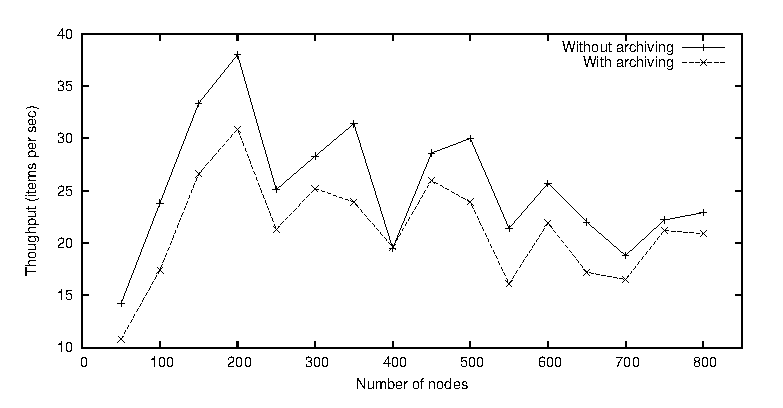
\epsfig{file=throughput.eps, width=\columnwidth}
\caption{Average throughput}
\end{center}
\end{figure}

\begin{figure}
\begin{center}
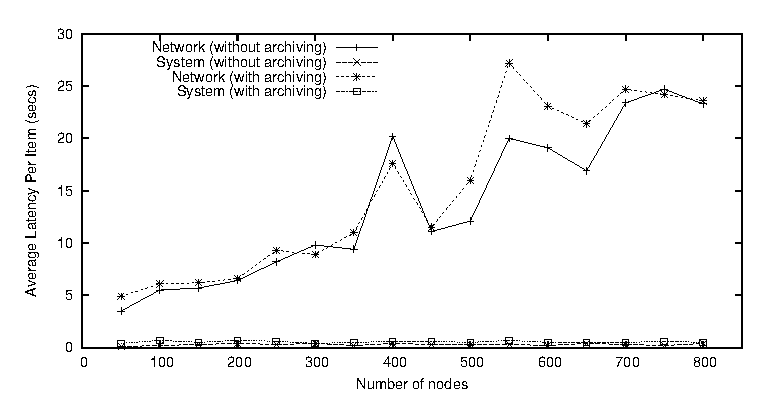
\epsfig{file=latency.eps, width=\columnwidth}
\caption{Average latencies per node}
\end{center}
\end{figure}


\begin{table*}
\begin{center}
\begin{tabular}{|l|r|r|r|r|r|r|r|r|r|r|r|r|}\hline
Num of nodes&	50&	100&	150&	200&	250&	300&	350&	400&	450&	500&	550&	600 \\ \hline\hline
Net latency per node (secs)&	9&	4&	4&	4&	8.6&	5.3&	19.1&	19.5&	14.4&	7.8&	12&	13.3 \\ \hline
Sys latency per node (secs)&	0&	0&	0&	0.3&	0.2&	0.4&	0.3&	0.1&	0.3&	0.4&	0.2&	0.7 \\ \hline
%Total Latency (secs)&	9&	4.04&	4&	4.3&	8.8&	5.8&	19.4&	19.6&	14.7&	8.2&	12.3&	14 \\ \hline
Total fetch time (secs)&	9&	5&	4&	5&	23&	9&	22&	23&	26&	14&	27&	28 \\ \hline	
Throughput (items/sec)&	5.6&	20&	37.5&	40&	10.9&	33.3&	15.9&	17.4&	17.3&	35.7&	20.4&	21.4 \\ \hline
\end{tabular}
\end{center}
\caption{Performance of Comon with no archiving}
\end{table*}


\begin{table*}
\begin{center}
\begin{tabular}{|l|r|r|r|r|r|r|r|r|r|r|r|r|}\hline
Num of nodes&	50&	100&	150&	200&	250&	300&	350&	400&	450&	500&	550&	600 \\ \hline\hline
Net latency per node (secs)&	16&	4&	4&	4&	18.9&	6&	20.6&	22&	8.4&	13&	21.8&	21.3 \\ \hline
Sys latency per node (secs)&	0.8&	1.28&	1.4&	1.8&	1.9&	1.5&	1.6&	1.3&	1.9&	1.7&	1.7&	2.2 \\ \hline
%Total Latency (secs)&	16.8&	5.28&	5.4&	5.8&	20.8&	7.5&	22.2&	23.3&	10.3&	14.7&	23.56&	23.5 \\ \hline
Total fetch time (secs)&	17&	6&	7&	7&	27&	12&	27&	30&	19&	33&	43&	43 \\ \hline
Throughput (items/sec)&	2.9&	16.7&	21.4&	28.6&	9.3&	25&	13&	13.3&	23.7&	15.2&	12.8&	14 \\ \hline
\end{tabular}
\end{center}
\caption{Performance of Comon with archiving}
\end{table*}


\section{Related Work}
\label{sec:related-work}

\section{Conclusions and Future Work}
\label{sec:conclusion}

\end{document}
